\documentclass[a4paper, 12pt]{article}
\usepackage[UTF8]{ctex}
% \usepackage[T1]{fontenc}
% \usepackage{inconsolata}


\usepackage{amsmath}
\usepackage{enumitem}
\setlist{
    nolistsep, % 去掉 item 和正文之间的间隔
    % labelindent=\parindent,
    leftmargin=*, % 保证小节标签缩进和上面对齐
    % labelsep=1em, % 标签后的空白
    align=left, % 标签对齐段落左边缘
}
\usepackage{tabularx}

\usepackage{graphicx}

\usepackage{geometry}
\geometry{
    a4paper,
    left=2cm,
    right=2cm,
    top=2cm,
    bottom=2cm,
}

\newcommand{\fs}[1]{\fontsize{#1 pt}{0pt}\selectfont}

\usepackage{mathtools}
\DeclarePairedDelimiter{\ceil}{\lceil}{\rceil}
\DeclarePairedDelimiter\floor{\lfloor}{\rfloor}

\usepackage{setspace}
% \setlength\parindent{0pt}
\setlength{\parindent}{2em} % 中文

% \newfontfamily\csl{Consolas}

\usepackage{array}
\newcolumntype{T}{>{\ttfamily}l}
\newcolumntype{Y}{>{\footnotesize\ttfamily}l}
\newcolumntype{y}{>{\footnotesize\ttfamily}c}

\usepackage{longtable}

\newcommand*{\thead}[1]{\multicolumn{1}{c}{\bfseries #1}}
\newcommand*{\yhead}[1]{\multicolumn{1}{c}{\footnotesize\bfseries #1}}

\newcommand{\ssa}{\phantom{x}}
\newcommand{\ssb}{\phantom{xx}}
\newcommand{\ssc}{\phantom{xxx}}
\newcommand{\ssd}{\phantom{xxxx}}
\newcommand{\sse}{\phantom{xxxxx}}

\usepackage{xcolor}
\usepackage{listings}
\definecolor{mygreen}{RGB}{28,172,0} % color values Red, Green, Blue
\definecolor{mylilas}{RGB}{170,55,241}

\newcommand{\ttf}{\ttfamily}

\lstdefinestyle{plainText}{language={},
    % basicstyle=\footnotesize \ttfamily,        % set font type and size
    basicstyle=\ttfamily,        % set font type and size
    breaklines=true,
    keywordstyle=\color{blue},
    % morekeywords={matlab2tikz},
    % morekeywords=[2]{1}, 
    % keywordstyle=[2]{\color{black}},
    identifierstyle=\color{black},
    stringstyle=\color{mylilas},
    % stringstyle=\color{purple},
    frame=single,
    framexleftmargin=0em,
    aboveskip=-\baselineskip,
    commentstyle=\color{mygreen},
    showstringspaces=false,% without this there will be a symbol in the places where there is a space
    % numbers=left,
    numbers=none,
    numberstyle={\tiny \color{black}}, % size of the numbers
    numbersep=9pt, % this defines how far the numbers are from the text
    tabsize=4,                     % sets default tabsize to 4 spaces
    emph=[1]{},
    emphstyle=[1]\color{red}, %some words to emphasise
    %emph=[2]{word1,word2}, 
    % emphstyle=[2]{style}, 
    escapeinside=``,               % Characters escape: To Use Chinese in codes   
}

\lstdefinestyle{myC}{language={C},
    % basicstyle=\footnotesize \ttfamily,        % set font type and size
    basicstyle=\ttfamily,        % set font type and size
    breaklines=true,
    keywordstyle=\color{blue},
    % morekeywords={matlab2tikz},
    % morekeywords=[2]{1}, 
    % keywordstyle=[2]{\color{black}},
    identifierstyle=\color{black},
    stringstyle=\color{mylilas},
    % stringstyle=\color{purple},
    frame=single,
    framexleftmargin=0em,
    aboveskip=-\baselineskip,
    commentstyle=\color{mygreen},
    showstringspaces=false,% without this there will be a symbol in the places where there is a space
    % numbers=left,
    numbers=left,
    numberstyle={\tiny \color{black}}, % size of the numbers
    numbersep=9pt, % this defines how far the numbers are from the text
    tabsize=4,                     % sets default tabsize to 4 spaces
    emph=[1]{printf},
    emphstyle=[1]\color{blue}, %some words to emphasise
    %emph=[2]{word1,word2}, 
    % emphstyle=[2]{style}, 
    escapeinside=``,               % Characters escape: To Use Chinese in codes   
}

\begin{document}
\begin{center}
{\fs{15}\bfseries {计算机动画原理与技术 ~作业 2 ~报告}}

\vspace{0.5\baselineskip}

{\fs{14} \kaishu 于泽汉 \hspace{1em} \textsf{No.118039910141}}
\end{center}

在本次实验中,对于三种不同的数值积分方法,可以分析观察得到如下结论:

\begin{itemize}[leftmargin=2em, label={}]
\item \textbf{精度:}欧拉法的精度较差,而且当步长提高时,误差也会增加;中点法精度稍高一些,误差相较欧拉法要小很多;龙格-库塔法的精度最高。

\item \textbf{稳定性:}欧拉法的稳定性较差,受不同参数变化影响较大;中点法稳定性稍好一些,积分结果的波动随参数变化相对较小;龙格-库塔法的稳定性最好,不同参数对积分结果的影响很小。

\item \textbf{运算速度:}欧拉法最快,中点法其次,龙格-库塔法最慢。

\end{itemize}

\vspace{\baselineskip}

\textbf{\fs{15}A. Ballistic Motion}

\begin{itemize}[leftmargin=2em, label={}]

\item 三种方法的实现效果和对应代码见 \texttt{hw2\_ballistic\_motion.html}。\\
浏览器(推荐使用 Chrome)打开可查看动画,文本编辑器打开可查看代码。\\
这里为了突出效果,步长选取为 0.02。

\begin{center}
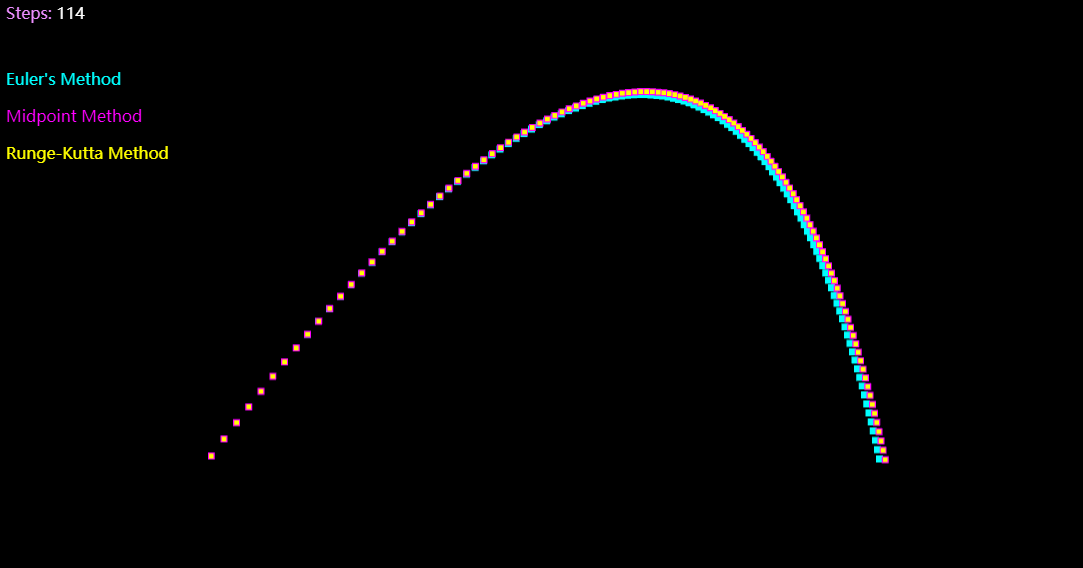
\includegraphics[width=\textwidth]{images/ballistic_motion.png}\\
三种不同的数值积分方法对应的炮弹抛射轨迹
\end{center}

\end{itemize}


\textbf{\fs{15}B. Spring-Mass Simulator}

\begin{itemize}[leftmargin=2em, label={}]

\item 三种方法的实现效果和对应代码见 \texttt{hw2\_spring\_mass.html}。\\
浏览器(推荐使用 Chrome)打开可查看动画,文本编辑器打开可查看代码。\\
这里为了突出效果,步长选取为 0.05。\\
这里选取了两组不同的 $k$ 和 $m$ 以观察效果。

\begin{center}
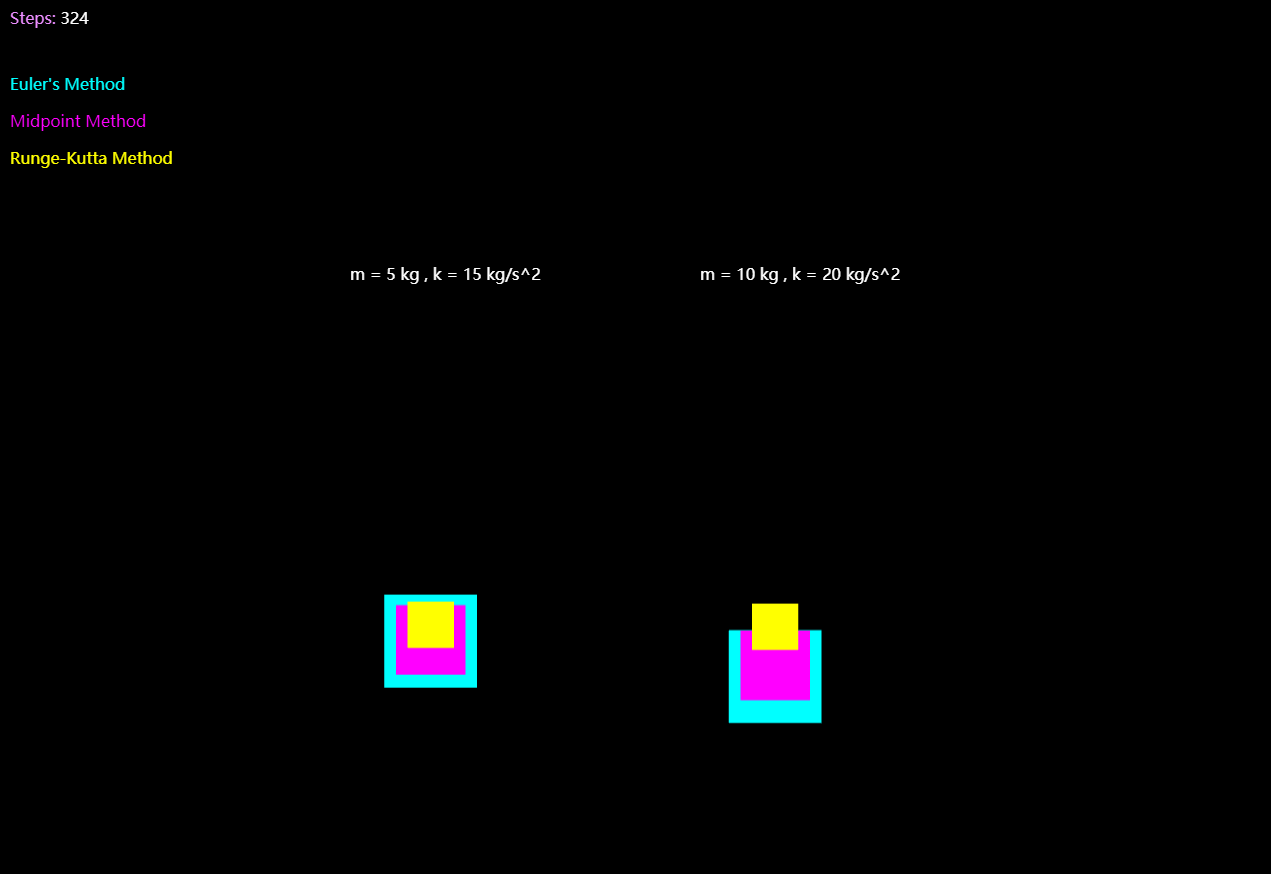
\includegraphics[width=\textwidth]{images/spring_mass.png}\\
三种不同的数值积分方法对应的弹簧-质量系统
\end{center}


\end{itemize}

\end{document}